\documentclass[a4paper,11pt]{article}

\usepackage{amsmath, amssymb, amstext, amsfonts, mathrsfs}


% \sffamily %schrift ohne Serifen

\usepackage[T1]{fontenc} 
% schriftencodierung f�r umlaute, trennung
% f\"ur Uni
\usepackage[latin1]{inputenc}
\usepackage{selinput}
% \usepackage[utf8x]{inputenc} 
\usepackage{bibgerm} 
% german bibliography
\usepackage[german]{babel}
%wichtig f�r deutschen Content
\usepackage{ucs}
%erweiterte UTF-8 Unterst�tzung
\usepackage{wrapfig} 
% Paket zur Positionierung einbinden
\usepackage{multirow}
% zusammenfassen von Tabellenzellen
% \usepackage{subscript}
% zum tiefstellen
\usepackage{lscape}
\usepackage{pdflscape}
% zum drehen der Seite
% \usepackage[super]{natbib}
\usepackage[square,sort,comma,numbers]{natbib}
% Erstellung es Literaturverzeichnisses
\usepackage{url}
% Umbruch f�r URL
\usepackage{pst-3dplot}
% f�r tex Grafiken n�tig
\usepackage{pstricks}
\usepackage{listings}
% f�r das einf�gen von Quelltext
\definecolor{codegray}{rgb}{0.92,0.92,0.92}
\lstset{basicstyle=\fontsize{9}{11}\selectfont\ttfamily, breaklines=true, backgroundcolor=\color{codegray}, numbers=left, numberstyle=\tiny, tabsize=4, language=java}
\definecolor{mymauve}{rgb}{0.58,0,0.82}
\definecolor{mygreen}{rgb}{0,0.6,0}
\lstset{
commentstyle=\color{mygreen},
keywordstyle=\color{mymauve},
language=Java,
stringstyle=\color{blue}
}


%Einstellungen f�r Quellcode
\usepackage[a4paper, left=3cm, right=2cm, top=2cm]{geometry}
% Formatierung R�nder
\usepackage[section]{placeins}
% f�r Floatbarriere
\usepackage{color}
\usepackage{colortbl}
%f�r die Verwendung von Farben

\clubpenalty = 10000 
\widowpenalty = 10000
\displaywidowpenalty = 10000
%Verhinderung von Hurenkindern und Schusterjungen
%10000 bedeutet die sie sollen kommplett vermieden werden

\title{Entwicklung einer Android-Applikation f�r die Alarmierung der Einsatzkr�fte der Freiwilligen Feuerwehren}

\author{Sebastian Rieger}

\pagenumbering{arabic}
%Seitenzahlen(arabische Zahlen)

\setlength{\parindent}{0.25cm} 
%Absatzeinzug �ndern in Zoll
\setlength{\parskip}{0.25cm}
%Absatzabstand
\linespread {1.5}
%Zeilenabstand

\usepackage{setspace}
\usepackage{hyperref}
%anklickbare Hyperlinks

%funktioniert nicht bei Fu�noten
\usepackage{graphicx}
\usepackage{graphics}
%f�r einbinden von Grafiken

\usepackage{framed}
%f�r Umrandung der Erkl�rung
\usepackage{acronym}
% f�r abk�rzungen
% \usepackage{PSTricks}
\usepackage{epstopdf}
% f�r eps bilder nutze pdflatex --shell-escape this.tex
\usepackage{amssymb}
% f�r mathematische Symbole

\usepackage{hyperref}
% klickbare links

% \usepackage{pdfpages}
\usepackage{rotating}
\usepackage{svg}
%%%%%%%%%%%%%%%%%%%%%%%%%%%%%%%%%%%%%%%%%%%%%%%%%%%%%%%%%%%%%%%%%%%%%%%%%%%%%%%%%%%%%%%%%%%%%%%%%%%%%
%% Angaben zur Arbeit
%%%%%%%%%%%%%%%%%%%%%%%%%%%%%%%%%%%%%%%%%%%%%%%%%%%%%%%%%%%%%%%%%%%%%%%%%%%%%%%

\newcommand{\Autor}{Sebastian Rieger}
\newcommand{\MatrikelNummer}{10286908}
\newcommand{\Kursbezeichnung}{TINF12B1}

\newcommand{\FirmenName}{PDV Systeme}
\newcommand{\FirmenStadt}{Erfurt}
\newcommand{\FirmenLogoDeckblatt}{{\includegraphics[width=3cm]{}}}

% Falls es kein Firmenlogo gibt:
%  \newcommand{\FirmenLogoDeckblatt}{}

\newcommand{\BetreuerFirma}{Prof. Rolf Kruse}
\newcommand{\BetreuerDHBW}{Prof. Steffen Avemarg}
\newcommand{\Titel}{Entwicklung eines Natural User Interface mit Hilfe moderner AR und AI Technologien}
\newcommand{\AbgabeDatum}{15.11.2017}

\newcommand{\Dauer}{24 Wochen}

% \newcommand{\Abschluss}{Bachelor of Engineering}
\newcommand{\Abschluss}{Master of Science}

\newcommand{\Studiengang}{Angewandte Informatik}
% \newcommand{\Studiengang}{Angewandte Informatik}
\newcommand{\Was}{Masterarbeit}

%%%%%%%%%%%%%%%%%%%%%%%%%%%%%%%%%%%%%%%%%%%%%%%%%%%%%%%%%%%%%%%%%%%%%%%%%%%%%%%%%%%%%%%%%%%%%%%%%%%%% 
%steuervariable
\usepackage{ifthen} %Package f�r if/else
\newboolean{bilder} %Deklaration
\setboolean{bilder}{true} %Zuweisung
% \setboolean{bilder}{false} %Zuweisung
%%%%%%%%%%%%%%%%%%%%%%%%%%%%%%%%%%%%%%%%%%%%%%%%%%%%%%%%%%%%%%%%%%%%%%%%%%%%%%%%%%%%%%%%%%%%%%%%%%%%%

\lstdefinelanguage{JavaScript}{
  keywords={typeof, new, true, false, catch, function, return, null, catch, switch, var, if, in, while, do, else, case, break},
  keywordstyle=\color{blue}\bfseries,
  ndkeywords={class, export, boolean, throw, implements, import, this},
  ndkeywordstyle=\color{darkgray}\bfseries,
  identifierstyle=\color{black},
  sensitive=false,
  comment=[l]{//},
  morecomment=[s]{/*}{*/},
  commentstyle=\color{purple}\ttfamily,
  stringstyle=\color{red}\ttfamily,
  morestring=[b]',
  morestring=[b]"
}


\makeatletter
\newcommand\footnoteref[1]{\protected@xdef\@thefnmark{\ref{#1}}\@footnotemark}
\makeatother

\begin{document}

\begin{center}
\vspace*{-2cm}
\hfill
\includegraphics[width=4cm]{Bilder/logo_FHE}\\[1cm]
{\Huge \Titel}\\[2cm]
{\Huge\scshape \Was}\\[2cm]
% {\large f�r die Pr�fung zum}\\[0.5cm]
% {\Large \Abschluss}\\[0.5cm]
% {\large des Studienganges \Studiengang}\\[0.5cm]
{\large \Studiengang}\\[0.5cm]
{\large an der}\\[0.5cm]
{\large Fachhochschule Erfurt}\\[0.5cm]
{\large von}\\[0.5cm]
{\large\bfseries \Autor}\\[1cm]
{\large Abgabedatum \AbgabeDatum}
\vfill
\end{center}
\begin{tabular}{l@{\hspace{1cm}}l}
Bearbeitungszeitraum             & \Dauer                       \\
Matrikelnummer                   & \MatrikelNummer              \\
% Kurs                             & \Kursbezeichnung             \\
% Ausbildungsfirma                 & \FirmenName                  \\
%                                  & \FirmenStadt                 \\
Betreuer der Masterarbeit    & \BetreuerFirma               \\
Zweitbetreuer der Masterarbeit     & \BetreuerDHBW                \\
\end{tabular}

\newpage
%Seitenumbruch
%%%%%%%%%%%%%%%%%%%%%%%%%%%%%%%%%%%%%%%%%%%%%%%%%%%%%%%%%%%%%%%%%%%%%%%%%%%%%%
%% Descr:       Vorlage für Berichte der DHBW-Karlsruhe, Erklärung
%% Author:      Prof. Dr. Jürgen Vollmer, vollmer@dhbw-karlsruhe.de
%% $Id: erklaerung.tex,v 1.2 2010/07/22 13:30:27 vollmer Exp $
%%%%%%%%%%%%%%%%%%%%%%%%%%%%%%%%%%%%%%%%%%%%%%%%%%%%%%%%%%%%%%%%%%%%%%%%%%%%%%%

% In Bachelorarbeiten muss eine schriftliche Erklärung abgegeben werden. In allen anderen
% Arbeiten entf�llt diese. Hierin best�tigen die Studierenden, dass die Bachelorarbeit
% selbst�ndig verfasst und s�mtliche Quellen und Hilfsmittel angegeben sind. Diese Erkl�rung
% bildet das zweite Blatt der Arbeit. Der Text dieser Erkl�rung muss auf einer separaten Seite
% wie unten angegeben lauten.

\newpage
\thispagestyle{empty}
\begin{framed}
\begin{center}
\Large\bfseries Erkl\"arung
\end{center}

\noindent
Ich, \Autor, versichere hiermit, dass ich die vorliegende Masterarbeit mit dem
Thema
"`\Titel"'
selbstst�ndig und nur unter Verwendung der angegebenen Quellen und Hilfsmittel angefertigt
habe.

\vspace{3cm}
\noindent
\underline{\hspace{4cm}}\hfill\underline{\hspace{6cm}}\\
Ort~~~~~Datum\hfill Unterschrift\hspace{4cm}
\end{framed}

%%%%%%%%%%%%%%%%%%%%%%%%%%%%%%%%%%%%%%%%%%%%%%%%%%%%%%%%%%%%%%%%%%%%%%%%%%%%%%%
\endinput
%%%%%%%%%%%%%%%%%%%%%%%%%%%%%%%%%%%%%%%%%%%%%%%%%%%%%%%%%%%%%%%%%%%%%%%%%%%%%%%

\newpage
\begin{spacing}{0.9}

%Einf�gen Inhaltsverzeichnis
\tableofcontents
\newpage
\section{Abstract}
\newpage
\section{Einleitung}
In den letzten zwanzig Jahren hat sich die Bedienung von Computern grundlegend ge�ndert. Vor nicht all zu vielen Jahren gab es nur die M�glichkeit mit Hilfe von Maus und Tastatur mit einem Computer zu interagieren. 

Mit dem Aufkommen von Touch-Screens jedoch �nderte sich auch die Benutzung von Computern. Es war nun m�glich, direkt mit dem Bildschirm zu interagieren ohne den Umweg �ber die Maus.

Als dann wenig sp�ter die ersten Sprachsteuerungen auf den Markt kamen, �nderte sich die Interaktion mit dem Computer erneut. So ist es nun m�glich, Computern mittels Sprache Befehle zu erteilen oder Texte zu sprechen, welche automatisch transkribiert werden.

Heute ist es mit manchen Smartphones schon m�glich, Nachrichten wie SMS zu schreiben und zu versenden, ohne das Telefon �berhaupt in die Hand zu nehmen. Dies ist nur durch neuste Entwicklungen in der \ac{KI} m�glich.

Im selben Zeitraum hat sich parallel auch die \ac{VR} entwickelt. Sie versucht Menschen mit Hilfe von verschiedenen Brillen in eine virtuelle Welt zu versetzen. Die Entwicklungen solcher \ac{VR} Systeme wurde vor allem von der Spieleindustrie getrieben, da sie immer neue Versuche unternimmt, Spieler besser in die Welt des Spiels zu versetzen. 

Eine Abstufung der \ac{VR} ist die \ac{AR}, welche versucht die analoge, reale Welt um digitale Inhalte zu erweitern. Hierbei sind die M�glichkeiten f�r den Einsatz von \ac{AR} fast unbegrenzt. 
Es ist also quasi m�glich, jede menschliche T�tigkeit durch die \ac{AR} zu unterst�tzen. 

Genau hier setzt der Schwerpunkt der Arbeit an. Im Verlauf soll versucht werden, ein \ac{NUI} unter Zuhilfenahme moderner \ac{AR} und \ac{KI} Technologien zu erstellen.

Hierf�r werden aktuelle \ac{AR} und \ac{KI} Systeme daraufhin untersucht, wie sie im Zusammenspiel ein \ac{NUI} bilden k�nnen, welches allein durch Sprache und Gesten mit einem Computer interagiert.

Es soll eine �bliche T�tigkeit mit Hilfe einer \ac{AR} Technologie in der realen Welt abgebildet werden, welche dann von einem Menschen nur unter Zuhilfenahme von Sprache und Gesten gesteuert und bearbeitet werden kann.
\newpage
\section{Natural User Interfaces}
Als Natural User Interfaces \ac{NUI} werden Benutzeroberfl�chen von Computern und Programmen bezeichnet, welche sich durch Gesten, Sprache, Ber�hren, Tippen und Wischen bedienen lassen. In der heutigen Zeit begegnen wir st�ndig solchen \ac{NUI}s. Zum Beispiel beim mehrmals t�glichen Griff zum Smartphone oder der Smartwatch. �ber einen ber�hrungsempfindlichen Display, werden Apps heute schon �ber Gesten gesteuert. \cite{InteraktiveSysteme}

Diese Steuerung funktioniert zum Teil bei der j�ngeren Generation, so genannten "`digital natives"', also Menschen die im digitalen Zeitalter geboren sind, schon automatisch und unterbewusst. Jeder, der schon einmal eine App bedient hat kennt die Geste zum l�schen aus einer Liste! Die Bewegung des Eintrags nach links oder rechts l�scht das entsprechende Element, getreu nach dem Motto "`Aus den Augen aus dem Sinn"'. \cite{WikiDigitalNativ}

Diese Art von Gesten ist so intuitiv f�r Menschen, das auch "`digital immigrants"', also Menschen, die erst im Erwachsenenalter den Umgang mit digitalen Ger�ten gelernt haben diese nach einmaliger Erkl�rung gelernt haben.

Aber das nat�rliche Verhalten von uns Menschen geht noch viel weiter. Diese einmal auf einem Smartphone gelernte Geste in einer App, wird unterbewusst auch auf andere Applikationen �bertragen. Eine App, welche diese einfache und mittlerweile etablierte Geste nicht unterst�tzt wird umgehend Kritik ernten, da sie mit altbekanntem bricht und so ein "`Nat�rliches"' arbeiten nicht mehr gegeben ist.

\subsection{Nat�rliche Bedienung durch Gesten}
Was jedoch genau macht eine Geste "`Nat�rlich"'? Die Beantwortung dieser Frage ist im gleichen Ma�e Trivial, wie Komplex. 

Dies bedeutet, sobald einmal eine "`Nat�rliche Geste"' gefunden wurde, erscheint wie gegeben und wird nicht in Frage gestellt, weil sie ja "`Logisch"' ist. Das Komplexe ist jedoch solche "`logischen Gesten"` erst einmal zu finden. 

Hierf�r m�ssen viele Aspekte aus den Verhaltenswissenschaften beachtet werden:
\begin{itemize}
\item Arbeitswissenschaft
\item Psychologie
\item Soziologie
\item P�dagogik
\end{itemize}

Erg�nzend zu diesen Aspekten gibt es die EN ISO 9241, welche Richtlinien der Mensch-Computer-Interaktion beschreibt. Ins besondere der Teil 110 "'Grunds�tze der Dialoggestaltung"` kann Helfen passende Bedienm�glichkeiten f�r ein \ac{NUI} zu finden. \cite{ISO9241} Die Grunds�tze sind:

\begin{itemize}
\item Aufgabenangemessenheit - geeignete Funktionalit�t, Minimierung unn�tiger Interaktionen 
\item Selbstbeschreibungsf�higkeit - Verst�ndlichkeit durch Hilfen / R�ckmeldungen 
\item Steuerbarkeit - Steuerung des Dialogs durch den Benutzer 
\item Erwartungskonformit�t - Konsistenz, Anpassung an das Benutzermodell 
\item Fehlertoleranz - unerkannte Fehler verhindern nicht das Benutzerziel, erkannte Fehler sind leicht zu korrigieren 
\item Individualisierbarkeit - Anpassbarkeit an Benutzer und Arbeitskontext 
\item Lernf�rderlichkeit - Minimierung der Erlernzeit, Metaphern, Anleitung des Benutzers 
\end{itemize}

\subsection{Erstellung eines Use Cases}
Anhand dieser Grunds�tze kann nicht nur ein System, welches mit Tastatur und Maus bedient wird definiert werden, sondern auch ein \ac{NUI}. Dies wird nun Beispielhaft an der Geste f�r "'l�schen"` gezeigt um sicher zu Stellen, dass im sp�teren Verlauf der Arbeit ein \ac{NUI} anhand genau dieser Grunds�tze definiert werden kann.

\paragraph{Aufgabenangemessenheit} 
Das Wischen zum L�schen eines Eintrags ist schnell und einfach zu erlernen. Ebenso kann die Geste schnell wiederholt werden um m�glichst schnell auch mehrere Elemente l�schen zu k�nnen.

\paragraph{Selbstbeschreibungsf�higkeit}
Die Geste ist zwar einfach und mittlerweile auch bekannt, aber es muss auch sichergestellt sein, dass neue Nutzer die Geste lernen k�nnen. Dies kann zum Beispiel durch ein kurzes wackeln beim ersten �ffnen angezeigt werden. Dem Nutzer wird durch diese Bewegung suggeriert, dass diese Elemente bewegbar sind. 

\paragraph{Steuerbarkeit}
Wischt der Nutzer nun bewusst oder durch Neugier ausgel�st vom Wackeln das Element aus dem Bildschirm muss immer die M�glichkeit bestehen das Element wiederherstellen zu k�nnen. Dies ist nur konsequent, da eine so einfache Geste auch einmal versehentlich gemacht werden kann.

\paragraph{Erwartungskonformit�t}
Ist diese Geste einmal etabliert, muss sie konsequent in allen Listen implementiert sein, da es sonst zum Bruch der Erwartung kommt und der Nutzer unn�tiger verwirrt wird.

\paragraph{Fehlertoleranz} 
Zu Fehlertoleranz geh�rt das wiederherstellen eines Eintrags wie schon unter Steuerbarkeit beschrieben. Zus�tzlich kommt jedoch hinzu, das die Geste eventuell vom Ger�t falsch interpretiert wurden ist und der Nutzer gar nichts l�schen wollte. Auch in solchen f�llen muss eine Wiederherstellung m�glich sein.

\paragraph{Individualisierbarkeit}
Das wischen ist eine tolle Geste! Aber in welche Richtung? Nach links oder rechts wischen zum l�schen? Genau hier muss die App schlau reagieren, denn die richtige Antwort ist: Beides muss m�glich sein. Bekanntlicher weise gibt es Links- und Rechtsh�nder, wobei das Ger�t zumeist mit der dominanten Hand gehalten wird. F�r einen Rechtsh�nder welcher den Daumen zum wischen links hat, ist das Wischen nach rechts leichter als nach links. Genau umgekehrt ist es bei Linksh�ndern. Diese wischen eher nach Links. 

Dieses Verhalten kann auch selbst nachgestellt werden, egal ob der Nutzer Links- oder Rechtsh�nder ist. Die Geste wird unterbewusst durch beide H�nde in unterschiedliche Richtungen ausgef�hrt. 

\paragraph{Lernf�rderlichkeit}
Bei der  Lernf�rderlichkeit trifft ganz klar das Sprichwort "'Aus den Augen aus dem Sinn"` zu. Der Nutzer m�chte etwas "'weg"` haben. Warum es also nicht au�erhalb des Displays platzieren. Es wird nicht mehr gesehen und ist somit "'weg"`. Diese einfache Analogie ist f�r jeden Nutzer zu verstehen und umzusetzen.

\subsection{Auswertung des Use Cases}
Anhand des vorgestellten Use Cases wurde gezeigt, dass es m�glich ist ein \ac{NUI} zu designen. Hierbei m�ssen nat�rlich die Gegebenheiten des jeweiligen Ger�tes beachtet werden, wie zum Beispiel das ein Smartphone in beiden H�nden gehalten werden kann. Dadurch kann sich gegebenen Falls der Use Case erweitern oder ver�ndern. 

1991 beschrieb Mark Weiser schon, wie sich Computer immer mehr in unseren Alltag integrieren und langsam immer unkenntlicher werden. Die Grenze zwischen realer Umwelt und virtueller Welt verschwimmt heute immer mehr. \cite{Computer21}

Dies hat nat�rlich auch zur Folge, das sich die Schnittstelle zwischen Mensch und Computer st�ndig �ndert und weiterentwickelt. Musste man 1997 zu beginn von Google noch Stichworte mit Maus und Tastatur eingeben um das Internet zu durchsuchen, reicht heute schon ein Sprachbefehl. 

Der Computer wertet mit verschiedenen Algorithmen das gesprochene aus, und versucht dem Nutzer eine direkte Antwort zu geben, w�hrend man 1997 von Google eine Liste mit Webseiten bekam, auf welchen die Schlagworte zu finden waren. 
\newpage
\section{Augumented Reality}
\newpage
\section{Artificial Intelligence}
Als \ac{AI} oder im deutschen auch \emph{artifizielle Intelligenz} oder \emph{k�nstliche Intelligenz}, bezeichnet, in der Informatik, ein System welches eine Automatisierte Intelligenz besitzt. Eine eindeutige Definition f�r \ac{AI} gibt es nicht, da es schon in der Psychologie an einer genauen Definition mangelt. \cite{WikiKI}

In der heutigen Zeit werden Systeme und Algorithmen die auf neuronalen Netzen basieren als ann�hernd intelligent bezeichnet. Ein Beispiel hierf�r ist "`Google Translate"' welches zwischen verschiedenen Sprachen mittels neuronalen Netz �bersetzt. \cite{TranslateKI}

Es gibt aber auch intelligente Systeme wie "`IBM Watson"', welche nicht auf neuronalen Netzen basieren und ann�hernd intelligent wirken. Diese Intelligenz ist das Resultat einer sehr gro�en Wissensbasis und verschiedenen kombinatorischen Algorithmen. Um zu zeigen wie Leistungsf�hig Watson ist, trat er 2011 in der Quizshow "`Jeopardy"' an und gewann gegen die weltbesten Spieler. \cite{IBMWatson}

\subsection{Sprachassistenten}

Im allgemeinen Sprachgebrauch werden als \ac{AI} die heute �blichen Sprachassistenten wie Siri, Alexa, Cortana oder Google Assistent bezeichnet. Das im Verlauf der Arbeit zu entwickelnde \ac{NUI} soll auf einen dieser Assistenten aufbauen.

Die Entwicklung einer eigenen Spracherkennung ist im Rahmen dieser Arbeit nicht m�glich, da dies sehr viel Zeit und Arbeit in Anspruch nimmt. Selbst Firmen wie Google oder Amazon ben�tigten mehrere Jahre um ihre Assistent auf das aktuelle Leistungsniveau zu heben.

\subsection{Funktionsweise der Sprachassistenten}
Auch wenn die genauen Implementierungen der Sprachassistenten verschiedenen ist, so haben sie alle eins gemenisam und zwar ist dies der Weg der Sprachverarbeitung.

Die Funktionsweise von Siri udn Co. ist recht einfach gehalten. Der Nutzer l�st mit einem Stichwort, "`Hey, Siri..."', "`Ok, Google..."' (Abbildung \ref{assistent_img} 1.)und so weiter, die Benutzung aus. Der darauf folgende Sprachbefehl wird aufgezeichnet und komprimiert an einen Server weitergeleitet (Abbildung \ref{assistent_img} 2.), welcher den gesprochenen Text auswertet und in schriftliche Befehle umwandelt (Abbildung \ref{assistent_img} 3.). Diese Befehle werden dann umgehend zur�ck an das Endger�t des Nutzers Versand (Abbildung \ref{assistent_img} 4.), welches nun auf die Befehle reagieren kann (Abbildung \ref{assistent_img} 5.). In Abbildung \ref{assistent_img} ist dieses vorgehen noch einmal schematisch Dargestellt. \cite{AIGrundlagen}

?????\textcolor{red}{ Wie sieht es besser aus? Verweis auf Abb. oder einzelnen Punkte angeben? oder punkte ganz weglassen? }?????

\begin{figure}[!ht]
\centering
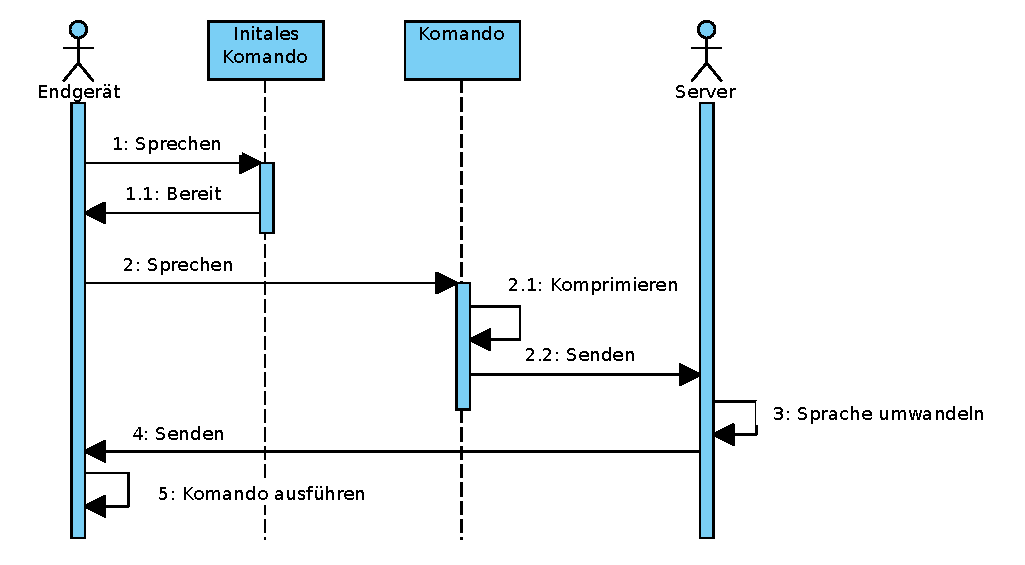
\includegraphics[width=14cm]{Bilder/Assistenten.eps}
\caption{Schematische Darstellung der Kommunikation von Sprachassistenten}
\label{assistent_img}
\centering
\end{figure}

\FloatBarrier

Hierbei ist zu beachten, dass jegliche Kommunikation zwischen Endger�t und Server bei allen Assistenten �ber HTTPS gesichert ist.

Innerhalb der Server, welche die Sprache zu Text wandeln, kommen fast immer neuronale Netze zum einsatz, da nur sie in der Lage sind schnell und eindeutig die Spachbefehle zu wandeln.
Durch die geh�ufte Verwendung mit immer neuen Stimmen und Befehlen lernen die Systeme immer mehr hinzu und k�nnen so die Anfragen immer schneller und besser umwandeln. Dies hat zur Folge, das ein System besser wird, je h�ufiger es genutzt wird.

In den nun folgenden Abschnitten werden die genannten Assistenten auf ihre M�glichkeiten untersucht.

\subsection{Untersuchung der Sprachassistenten}
Es soll nun untersucht werden, in wie weit die heute g�ngigen Assistenten genutzt werden k�nnen, um eine Sprachsteuerung f�r ein \ac{NUI} (siehe Kapitel ?????) umzusetzen.

Hierbei muss der Assistent folgende Kriterien erf�llen:
\begin{itemize}
 \item Lauff�gig auf der Microsoft HoloLens
 \item Offene Programmierschnittstelle (\ac{SDK})
 \item M�glichkeit eigener Sprachkomandos
\end{itemize}

\subsubsection{Siri}
Der wohl �lteste und bekannteste Sprachassistent ist "`Siri"'. Siri ist eine Software zur Spracherkennung und wurde von Apple im Jahre 2010 zusammen mit der Firma Siri Inc. von Apple aufgekauft. Schon ein Jahr sp�ter wurde der Assistent im Zuge der Ver�ffentlichung des iPhone 4s vorgestellt und ver�ffentlicht.

Siri ist eine propriet�re Software und nur iOS, machOS, watchOS und tvOS einsetzbar, weshalb eine Verwendung auf der HoloLens nicht m�glich ist. Zwar verf�gt Siri �ber ein offenes \ac{SDK}, dieses ist jedoch nur f�r Apple eigene Betriebssysteme ausgelegt. \cite{SiriKit} \cite{SiriKit2}


\subsubsection{Alexa}
Alexa ist der Name des Sprachassistenten, welcher von Amazon entwickelt wird und im November 2014 ver�ffentlicht wurde. Seither entwickelt Amazon seinen digitalen Assistenten stetig weiter. 
\cite{WikiAlexa}

Grunds�tzlich funktioniert auch Alexa wie schon im Abschnitt ????? beschrieben. Alexa arbeitet mit sogenannten Skills. Diese erm�glichen es Entwicklern den Assistent mit neuen Funktionen zu erweitern. Will ein Nutzer diesen Skill verwenden, muss er ihn zun�chst innerhalb seines pers�nlichen Assistenten installieren. Danach beherrscht Alexa die entsprechenden Kommandos des Skills. \cite{AmzSkills}

Die eigentlichen Skills, also kleine Programme, welche innerhalb der Amazon Cloud ausgef�hrt und durch den Assistenten gestartet werden k�nnen entweder in Java oder Node.js geschrieben werden. Um diese sp�ter zu ver�ffentlichen muss der Entwickler �ber ein Amazon Developer Account verf�gen.

Amazon verfolgt zur Zeit eine gro�e Marketing-Offensive, welche f�r verschiedene Produkte der Amazon Echo Serie, welche Alexa integriert haben.
Zus�tzlich ist es m�glich Alexa auch auf eigenen Ger�ten verf�gbar zu machen. Hierf�r wird das \ac{AVS} ben�tigt. Dieses \ac{SDK} erm�glicht es den Amazon Assistent auch auf Ger�ten verf�gbar zu machen, welche nicht von Amazon hergestellt wurden. \cite{AVS}

Mit den Skills und dem \ac{AVS}-\ac{SDK}, welches C++ basiert ist, ist es m�gliche alle Ger�te die ein Mikrofon besitzen mit dem Amazon Assistenten auszustatten.

Ein weiterer Vorteil von Alexa sind die sogenannten Speechcons. Diese werden speziell von Amazon zur Verf�gung gestellt, um eine m�glichst nat�rliche und vor allem richtig betonte Aussprache zu gew�hrleisten. Speechcons sind kurze Phrasen, welche in der Regel Umgangssprachlich genutzt werden, wie zum Beispiel der Ausspruch "`ich glaub mein Schwein pfeift"' oder "`Pustekuchen"'. Zus�tzlich steht mit "`Whispers"' auch ein Modus bereit, welcher Alexa fl�stern l�sst. \cite{GolemAlexa} \cite{Speechcons} 

All dies, macht Alexa zumindest f�r den Zuh�rer momentan zu den besten Assistenten auf den Markt.

\subsubsection{Cortana}
Nutzer von "`Windows 10"', einer Xbox oder eines Windows Phone kennen sie bereits, "`Cortana"', den digitalen Assistenten, welcher von Microsoft entwickelt wurde.  Er wurde im Jahr 2014 ver�ffentlicht und steht neben den genannten Microsoft Ger�ten auch f�r Android und iOS zur Verf�gung. Grunds�tzlich kann Cortana eine Suche starten, Programme ausf�hren oder Termine und Notizen verwalten. \cite{WikiCortana}

�ber Skills k�nnen Entwickler �hnlich wie bei Alexa zus�tzliche Funktionen erstellen und f�r Nutzer freigeben. Das von Microsoft bereitgestellte Skills Kit ist momentan noch nicht freigegeben und befindet sich aktuell in einer �ffentlichen Beta-Phase.

Skills f�r Cortana werden �hnlich wie die von Alexa in der Clound ausgef�hrt und k�nnen in .NET oder Node.js geschrieben werden. \cite{Cortana}

\subsubsection{Google Assistent}
Der Google Assistant ist ein Assistent, welcher von Google entwickelt wird und 2016 als Nachfolger von Google Now erschienen ist. \cite{GoogleAssistant}

Eine Besonderheit dieses Assistenten ist, das er Fragen auch aus dem Kontext fr�her gestellter Fragen beantworten kann. So kann ein Nutzer zum Beispiel Fragen "`In welchem Verein spielt Manuel Neuer?"'. Wenn als n�chstes die Frage "`Wie alt ist er?"' folgt, kann der Google Assistent aus dem Kontext schie�en, das ebenfalls "`Manuel Neuer"' als "`er"' gemeint ist. \cite{AssistantBild}

Der Google Assistant ist durch eine Vielzahl von \ac{SDK}s wie zum Beispiel Android, Apple, C++, Python und weitere unter quasi allen Plattformen lauff�hig. \cite{ApiAI}

Mit sogenannten "`Agents"' ist es m�glich, �hnlich wie mit Alexa Skills, �ber ein Web-Interface neue Funktionen zu erstellen.

\subsubsection{Auswertung der M�glichkeiten}
Nach dem �berblick �ber die vier Assistenten Siri, Alexa, Cortana und Google Assistent wird nun ausgewertet welcher am besten f�r die Erstellung eines \ac{NUI} geeignet ist.

Im Kapitel \ref{Augmented Reality} wurde die Microsoft Hololens f�r die Erstellung eines \ac{NUI} favorisiert. Auf ihr muss also der Assistent lauff�hig sein. Da Apple f�r Siri nur ein \ac{SDK} unter iOS bereitgestellt ist es nicht m�glich diesen Assistent auf der Hololens zu verwenden. Alexa, Cortana und der Google Assistant k�nnen auf der Hololens aufsetzen. Dies funktioniert durch die bereitgestellten \ac{SDK}s zumindest theoretisch und muss in der Praxisumsetzung der Arbeit noch einmal gepr�ft werden.

Alle Assistenten verf�gen �ber ein offenes \ac{SDK}, welches kostenlos verwendet werden kann. Lediglich bei der Ausf�hrung von Befehlen innerhalb der Cloud (Skills)  fallen kosten an. Hierbei rechnen alle Hersteller nach Anzahl der Ausf�hrungen ab und nicht nach Laufzeit oder Rechenleistung.

Siri, Alexa und der Google Assistant haben jeweils die M�glichkeit eigene Funktionen zu erstellen und diese innerhalb von Programmen zur Ausf�hrung zu bringen. Durch das Web-Interface des Google Assistant k�nnen zwar eine Vielzahl von Funktionen erstellt werden, jedoch sind die M�glichkeiten bei Alexa zumindest aktuell um ein vielfaches gr��er, da hier Java oder Node.js Quellcode zur Ausf�hrung kommt. 
Siri kann Befehle verarbeiten und Funktionen innerhalb einer installierten App aufrufen. Jedoch ist die Funktionalit�t hierauf beschr�nkt. Lediglich Apple kann eigene neue Funktionen f�r Siri bereitgestellen.

Microsoft arbeitet zur Zeit an einem Skill \ac{SDK} f�r Cortana, welches �hnlich wie der Amazon Ansatz aussieht. F�r Cortana kommt in der Cloud .NET oder Node.js Code zur Ausf�hrung. Aktuell befindet sich dieses \ac{SDK} in einer �ffentlichen Beta-Phase und die Schnittstellen sind noch nicht Final.

In der Tabelle \ref{Assistentenvergleich} ist dies noch einmal zusammengefasst.


\begin{table}[htbp]
\begin{center}
\begin{tabular}{|c|c|c|c|c|c|}
\hline
 Anforderung 					& Priorisierung & Siri				& Alexa				& Cortana 	 		& Google Assistant		\\ \hline		
 
 Lauff�gig auf der Microsoft HoloLens 		& sehr hoch 	& \textcolor{red}{X} 		& \textcolor{green}{\checkmark} & \textcolor{green}{\checkmark}	& \textcolor{green}{\checkmark} \\ \hline
 
 Offene Programmierschnittstelle (\ac{SDK})	& hoch 		& \textcolor{green}{\checkmark}	& \textcolor{green}{\checkmark} & \textcolor{green}{\checkmark} & \textcolor{green}{\checkmark} \\ \hline
 
 M�glichkeit eigener Sprachkomandos		& sehr hoch 	& \textcolor{green}{\checkmark}	& \textcolor{green}{\checkmark} & \textcolor{red}{X} 		& \textcolor{green}{\checkmark} \\ \hline
  
 
\end{tabular}
\end{center}
\caption{Tabellarischer Vergleich der Assistenten}
\label{Assistentenvergleich}
\end{table}

Aufgrund der vorangegangenen Analyse zeigte sich, das Alexa momentan die besten M�glichkeiten bietet um in ein \ac{NUI} integriert zu werden. Hierf�r spricht vor allem das \ac{AVS}-\ac{SDK} welches schnell kompiliert und einsatzbereit ist. Die zweite Wahl, w�re der Google Assistant mit seiner Vielzahl von \ac{SDK}s. Sollten beide M�glichkeiten technisch nicht umsetzbar sein, so muss auf Cortana zur�ckgegriffen werden. Hier ist eine Lauff�higkeit durch Microsoft garantiert. Jedoch ist das Skill \ac{SDK} noch nicht final ver�ffentlicht.
\newpage
\section{Beschreibung eines Natural User Interface}
Im foldenden Kapitel werden verschiedene m�gliche Einsatzgebiete f�r ein \ac{NUI} mit aktuellen \ac{AR} und \ac{AI}-Technologien beschireben. 
Anhand eines Einsatzgebietes wird dann ein \ac{NUI} genauer beschrieben und designed.

\subsection{Einsatzgebiete}
Um �berhaupt ein \ac{NUI} erstellen und beschreiben zu k�nnen, muss ein spezielles Szenario gew�hlt werden, an das Gesten und Sprachkommandos angepasst werden.

\subsubsection{Architektur Designer}
Schon heute gibt es unz�hlige Programme, mit den Geb�ude designt werden k�nnen. Eines davon ist "`Architekt 3D"' mit dem nicht nur Modelle erstellt werden k�nnen, sondern auch Grund- und Auf-risse erzeugt werden k�nnen.

\begin{figure}[!ht]
\centering
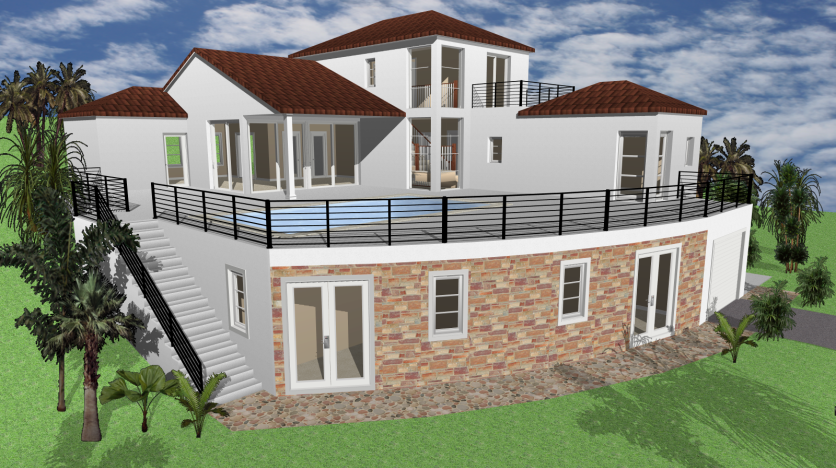
\includegraphics[width=10cm]{Bilder/architek_3d.png}
\caption{Darstellung eines Hauses in Architekt 3D \cite{Arch3D}}
\label{arch_3d}
\centering
\end{figure}

In Abbildung \ref{arch_3d} ist die Darstellung eines Hause zu sehen, welches mit "`Architekt 3D"' erstellt wurde. In einer \ac{AR}-Umgebung mit einem \ac{NUI} w�re es jetzt zum Beispiel m�glich, um das Geb�ude herum zu gehen. Es per Sprachbefehl vergr��ern oder verkleinern. Es k�nnte auch m�glich sein, zum Beispiel Leitungen einzublenden.

Mit Gesten k�nnte es zum Beispiel m�glich werden, Fenster und T�ren zu verschieben oder Objekte zu selektieren. 

Aber selbst das Designen von Grund auf ist innerhalb einer \ac{AR}-Anwendung kein Problem. �ber ein Sprachkommando k�nnten zum Beispiel W�nde ausgew�hlt werden, welche dann �ber Gesten im Raum gesetzt, verschoben oder gel�scht werden k�nnen.

Das System k�nnte �hnlich gestaltet wie zum Beispiel "`Google Blocks"' mit welchem es unter Verwendung der "`Oculus Rift"' oder der "`HTC Vive"' m�glich ist, 3D-Modelle zu erstellen.
\cite{Blocks}

\subsubsection{Bauen im Bestand}
Eine weitere Anwendungsm�glichkeit f�r ein verwandtes System w�re das Bauen im Bestand. Also, wenn schon bestehende H�user ver�ndert und modifiziert werden sollen. Mit Hilfe von Sprachbefehlen k�nnte man bestehende Strom oder Rohrleitungen unter den W�nden anzeigen um zu sehen, welche baulichen Ver�nderungen getroffen werden k�nnen und welche nicht. 

So ist es zum Beispiel m�glich neue Leitungen zu Planen ohne alte zu besch�digen oder suchen zu m�ssen. 

\begin{figure}[!ht]
\centering
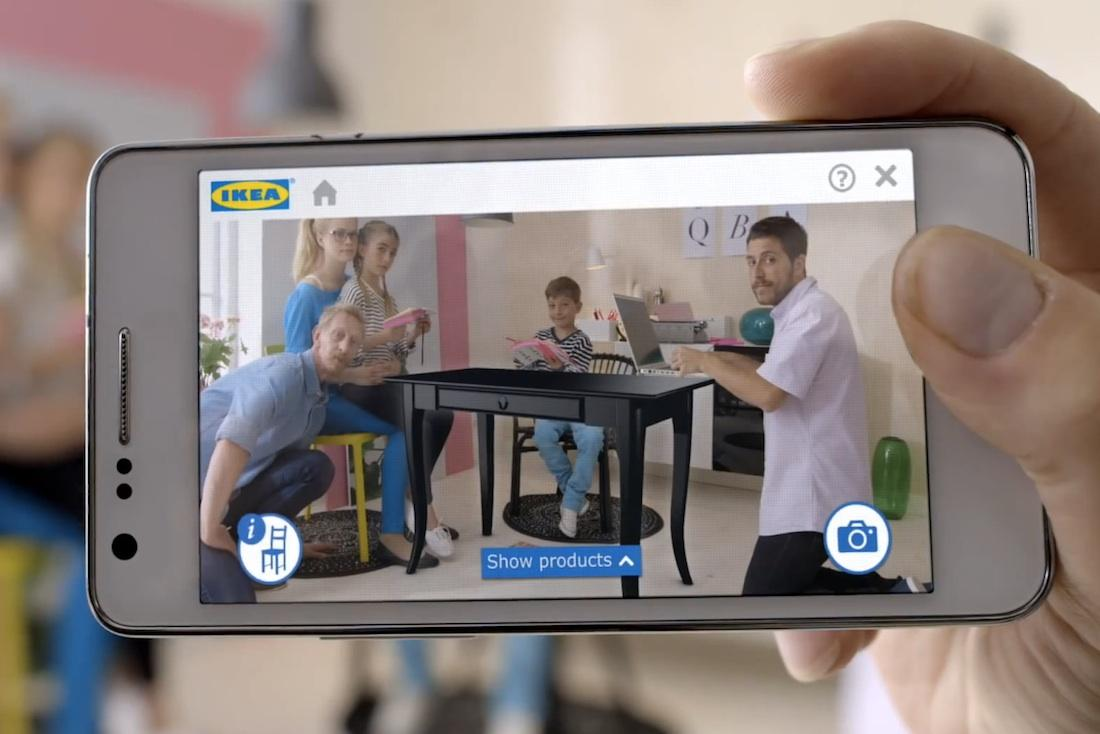
\includegraphics[width=10cm]{Bilder/ikea.jpg}
\caption{Ikea's \ac{AR} M�belst�cke \cite{IkeaVideo}}
\label{ikea_video}
\centering
\end{figure}

Es w�re m�glich, zum Beispiel K�chenzeilen in R�umen zu platzieren um zu sehen, wie diese Ausfallen und ob sie zum Raum passen. In dieser Technik Vorreiter ist Ikea. Seit 2014 k�nnen Kunden von Ikea den Katalog mit der Ikea eigenen App scannen und so M�belst�cke ausw�hlen, welche dann wiederum als \ac{AR}-Objekt in der eigenen Wohnung angesehen werden k�nnen. In Abbildung \ref{ikea_video} ist die Ikea-App zu sehen, in der Nutzer \ac{AR}-M�bel in ihrer Wohnung platzieren k�nnen.
\cite{Ikea}

\subsubsection{Unterst�tzung von Rettungskr�ften}
Feuerwehrleute r�cken t�glich aus, um unser aller Leben zu retten, sollten wir einmal in eine Gefahrensituation geraten. In stark verqualmten R�umen suchen Feuerwehrleute zum Beispiel nach �berlebenden. Hilfreich w�re hier zum Beispiel ein Ger�t, welches unter schlechter Sicht, den Raum Scannt und Hindernisse, wie Tische, Schr�nke oder aber weitere T�ren anzeigt. 

�ber Sprachbefehle w�re es zum Beispiel M�glich den Raum zu Scannen und zu Visualisieren. Eine andere M�glichkeit w�re es anhand von W�rmesignaturen nach �berlebenden zu suchen. 

Ein solcher Einsatz, liegt jedoch noch in weiter Ferne, da hierf�r Ger�te entwickelt werden, welche R�ume auch unter schlechter Sicht zuverl�ssig Scannen und zum anderen auch W�rmebilder verarbeiten k�nnen. 

Momentan sind Aktuelle \ac{AR}-Ger�te noch nicht in der Lage unter solchen Situation zu arbeiten. Geschweige den, das sie den harten Einsatz �berstehen w�rden. Denn Wasser, Staub, Hitze und harte St��e sind noch immer der Feind von solchen Ger�ten.

\subsubsection{Bestm�gliches Beispiel}
Es wurden drei m�gliche Beispiele beschrieben, Anhand von denen ein Prototyp entwickelt werden kann, welcher genau aufzeigt, in wie weit ein \ac{NUI} mit aktuellen \ac{AR} und \ac{AI} Technologien erstellt werden kann und welche St�rken und Schw�chen es hat.

Der dringendste Bedarf f�r eine Applikation h�tte mit Sicherheit die Feuerwehrleute, welche unter Einsatz ihres Lebens arbeiten. Leider gibt es f�r eine solche Anwendung noch keine Hardware. Nicht nur, das aktuelle \ac{AR}-Brillen heute nur bei guter Sicht arbeiten, sie verf�gen auch nicht �ber die M�glichkeit W�rmebilder zu erstellen. Weshalb dieser Ansatz nicht weiter verfolgt wird.

Das Bauen im Bestand mit \ac{AR} ist nat�rlich sehr n�tzlich. Jedoch ist das Rahmenwerk welches als Vorarbeit geleistet werden muss vom Umfang zu gro� f�r diese Arbeit. Es m�sste eine Raumerkennung entwickelt werden, welche zuverl�ssig T�ren und Fenster erkennt. Au�erdem erst Beispieldaten f�r Leitungsnetze von R�umen angelegt werden. 

Am besten eignet sich der Architektur Editor. Es ist heute relativ einfach m�glich, ein grundlegendes Design Programm zu erstellen, welches Objekte erstellen oder ver�ndern kann. 
Dieses System, kann dann um ein \ac{NUI} erweitert werden.

\subsection{Erstellung eines Architektur Editor als Prototyp}
Nat�rlich ist es innerhalb der Arbeit nicht m�glich einen realistischen Architektur Editor zu erstellen, mit dem es m�glich ist hochaufl�sende \ac{AR}-Modelle von Geb�uden zu designen.
Hierauf liegt auch nicht das Augenmerk der Arbeit. 

Umgesetzt werden, soll ein 3D-Designer, mit welchem es �hnlich wie im Spiel "`Minecraft"' m�glich ist, verschiedene \ac{AR}-Bl�cke in der realen Welt zu platzieren um hiermit  Gegenst�nde Designen zu k�nnen.

Der entstehende Prototypische Designer soll dann sp�ter nur �ber Gesten und Sprache gesteuert werden k�nnen. Hierf�r werden folgende Gesten und Sprachbefehle ben�tigt.

Gesten: 
\begin{itemize}
 \item Block setzen
 \item Block entfernen
 \item Objekt drehen
\end{itemize}

Sprachbefehle:
\begin{itemize}
 \item Block Material ausw�hlen
\end{itemize}

Es ergeben sich f�r den reinen Design Einsatz also drei Gesten und ein Sprachbefehl. Mit den Gesten ist es m�glich Bl�cke zu setzen, zu entfernen und das gesamte Objekt zu drehen. Mit einem Sprachbefehl, kann das Material der Bl�cke ge�ndert werden. 

Aber ein \ac{NUI} macht nicht nur aus, dass es mit Gesten und Sprache gesteuert werden kann. Es muss sich auch auf den Nutzer einlassen und Fehlertolerant sein. Das hei�t im Umkehrschluss, es muss auch m�glich sein Gesten durch Sprache zu ersetzen und umgekehrt. Hieraus ergeben sich weitere Gesten und Sprachbefehle

Gesten: 
\begin{itemize}
 \item Block Material ausw�hlen
\end{itemize}

Sprachbefehle:
\begin{itemize}
 \item Block setzen
 \item Block entfernen
 \item Objekt drehen
\end{itemize}

Es ergeben sich also aus vier Bedienm�glichkeiten acht M�gliche Bedienszenarien f�r das reine Designen. Ob alle M�glichkeiten umsetzt werden, wird sich in der sp�teren Bedienung herausstellen. Eventuell sind Gesten zum Ausw�hlen des Materials nicht Sinnvoll und Praktikabel ebenso wie das Setzen und Entfernen von Bl�cken. 

\newpage
\section{Versuch der Entwicklung eines Natural User Interface anhand der Microsoft HoloLens und ...}
\section{Fazit}
\section{Zusammenfassung}


\end{spacing}

\newpage
\section{Abk�rzungsverzeichnis}
\begin{acronym}
  \acro{KI}{\emph{k�nstliche Intelligenz}}
  \acro{VR}{\emph{Virtuelle Realit�t}}
  \acro{AR}{\emph{Augumented Reality}}
  \acro{NUI}{\emph{Natural User Interface}}
  \acro{AV}{\emph{Augmented Virtuality}}
  \acro{SDK}{\emph{Software Development Kit}}
  \acro{AI}{\emph{Artificial Intelligence}}
  \acro{AVS}{\emph{Amazon Voice Service}}
  \acro{SRGS}{\emph{Speech Recognition Grammar Specification}}
  \acro{W3C}{\emph{World Wide Web Consortium}}
  \acro{XML}{\emph{Extensible Markup Language}}
  \acro{UWP}{\emph{Universal Windows Plattform}}
\end{acronym}
\newpage
\listoffigures
\newpage
\listoftables
% Abk�rzungsverzeichnis
\newpage
\bibliographystyle{alpha}
% verzeichnis im DIN format
\bibliography{Quellen}
\end{document}
